\documentclass[10pt, a4paper]{article}
\usepackage[margin=4.2cm]{geometry}
\usepackage{setspace}
\onehalfspacing
\doublespacing
\usepackage[hidelinks]{hyperref}
\usepackage{placeins}
\usepackage{tikz}
\usetikzlibrary{arrows}
\usepackage{pgfplots}
\pgfplotsset{compat=newest}
\usepackage{pgfplotstable}
\usepgfplotslibrary{fillbetween}
\usetikzlibrary{matrix}
\iffalse
\usepackage{tikz}
\usetikzlibrary{arrows}
\usepackage{pgfplots}
\pgfplotsset{compat=newest}
\usepgfplotslibrary{clickable}
\fi
\usepackage[utf8x]{inputenc}
\usepackage{amsmath}
\usepackage{amsfonts}
\usepackage{amssymb}
\usepackage{graphicx}
\usepackage{caption}
\usepackage{subcaption}
\usepackage{sidecap}
\usepackage{multicol}
%\usepackage{dsfont}
%\usepackage{lipsum}

\author{
	\textbf{André Rodrigues, Germano Leite, Juliana Nunes}
}


\title{ \textbf{Projeto Final de Curso}}

\date{}

\renewcommand{\figurename}{Figura}
\renewcommand{\tablename}{Tabela}
\renewcommand\refname{Referências}

\tikzstyle{state}=[shape=circle,draw=blue!50,fill=blue!20,minimum size=1.0cm]
\tikzstyle{smallstate}=[shape=circle,draw=blue!50,fill=blue!20,minimum size=0.5cm]
\tikzstyle{observation}=[shape=rectangle,draw=orange!50,fill=orange!20]
\tikzstyle{lightedge}=[<-,dashed]
\tikzstyle{mainstate}=[state,thick]
\tikzstyle{mainedge}=[<-,thick]

\usepackage{mathtools}
\DeclarePairedDelimiter{\ceil}{\lceil}{\rceil}
\DeclarePairedDelimiter{\floor}{\lfloor}{\rfloor}


\begin{document}

\maketitle

\section{Introdução}
	\label{sec:introducao}
	Na medida em que o uso de sistemas computacionais aumenta na sociedade atual, aplicações com exigências de tempo real tornam-se cada vez mais comuns. Essas aplicações variam muito em relação à complexidade e às necessidades de garantia no entendimento de restrições temporais. Existem sistemas de tempo real simples, como os controladores inteligentes embutidos em utilidades domésticas, tais como lavadora de roupa e videocassetes e existem sistemas de complexidade maior, como os sistemas militares de defesa, sistemas de controle de plantas industriais (químicas e nucleares) e controle de tráfego aéreo e ferroviário.

Em aplicações de tempo real, também é importante ressaltar que existem sistemas que apresentam restrições de tempo mais rigorosas do que outras, por exem- plo, os sistemas responsáveis pelo monitoramento de pacientes em hospitais, sistemas embarcados em robôs e veículos (de automóveis até aviões) e há também sistemas que não apresentam restrições tão rigorosas, por exemplo, videogames, teleconferências através da internet e aplicações de multimídia. Todas essas aplicações que apresentam a característica adicional de estarem sujeitas a restrições temporais são agrupadas no que é usualmente identificado como Sistema de Tempo Real.

Diante dessa premissa, com o intuito de aplicar os conhecimentos adquiridos na disciplina de Sistemas de Tempo Real desenvolvemos neste projeto um robô que possui tarefas a serem executadas em tempo real.  Utilizamos a plataforma Arduino, diversos sensores e uma biblioteca para auxiliar no escalonamento de tarefas. Neste documento são detalhadas todas as etapas do desenvolvimento do robô. O documento foi organizado da seguinte forma: A seção 2 explica como o robô foi construído, a seção 3 apresenta as tarefas do robô e mostra como elas foram implementadas, a seção 4 expõe os resultados obtidos e por fim, a seção 5 apresenta a conclusão do trabalho. 

\section{Construção do Robô}
	\label{sec:trabRel}
	Para a construção estrutural do robô utilizamos materiais fornecidos gentilmente pelo Professor Douglas Macharet (UFMG/DCC) e também materiais adquiridos pelos alunos integrantes deste trabalho. Nas subseções 2.1 e 2.2 descrevemos os materiais e métodos utilizados para o desenvolvimento do robô

\subsection{Materiais}

Para arquitetar a estrutura do robô utilizamos peças de Lego (Figura \ref{lego1}). Um kit de peças de lego como esse têm como uma de suas finalidades a construção de robôs, oferecem uma grande quantidade de peças que facilitam o projeto e tornam mais prática a sua execução.

\begin{figure}[!htb]
	\centering
	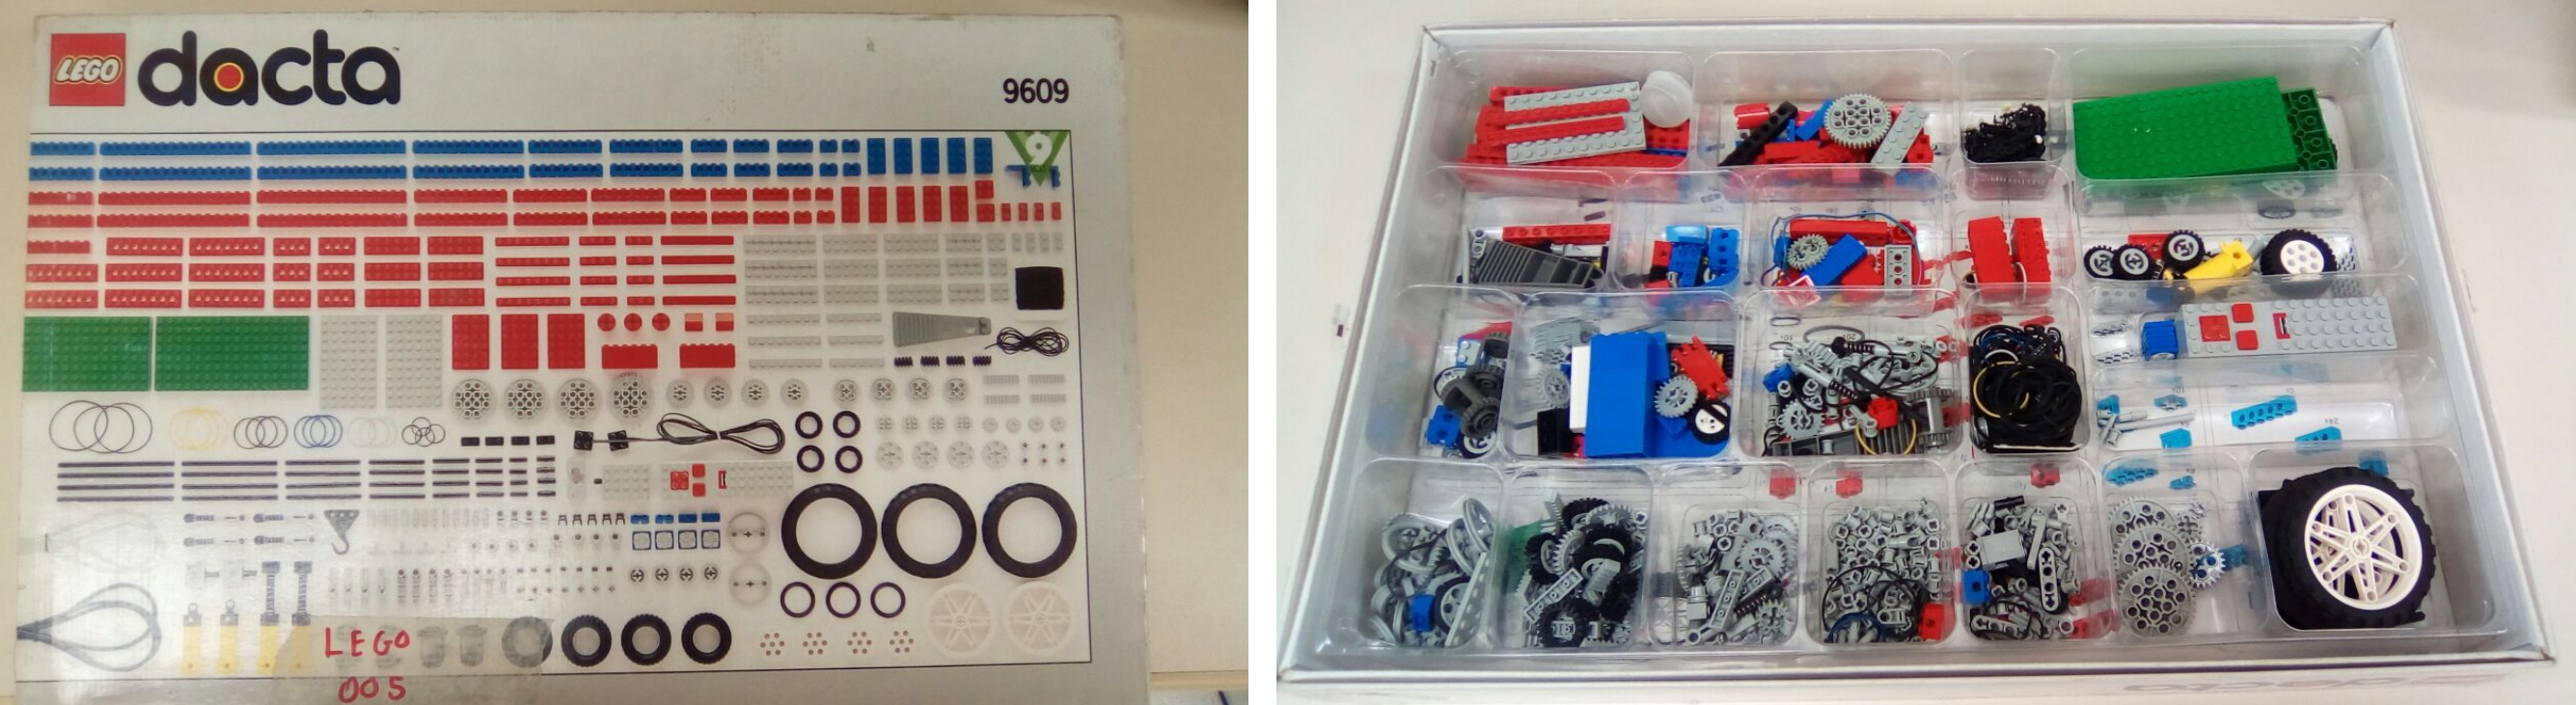
\includegraphics[width=12.5cm]{images/lego1.png}
	\caption{Kit de Lego.}
	\label{lego1}
\end{figure}

Para permitir que o robô realize as tarefas é necessário uma plataforma que permita integrar os sensores (Figuras \ref{sensores1}, \ref{sensores2}, \ref{sensores3} e \ref{sensores4}) que precisamos para a execução das mesmas. A plataforma escolhida foi o Arduino (Figura \ref*{arduino}), uma plataforma eletrônica de código aberto.


\begin{figure}[!htb]
	\centering
	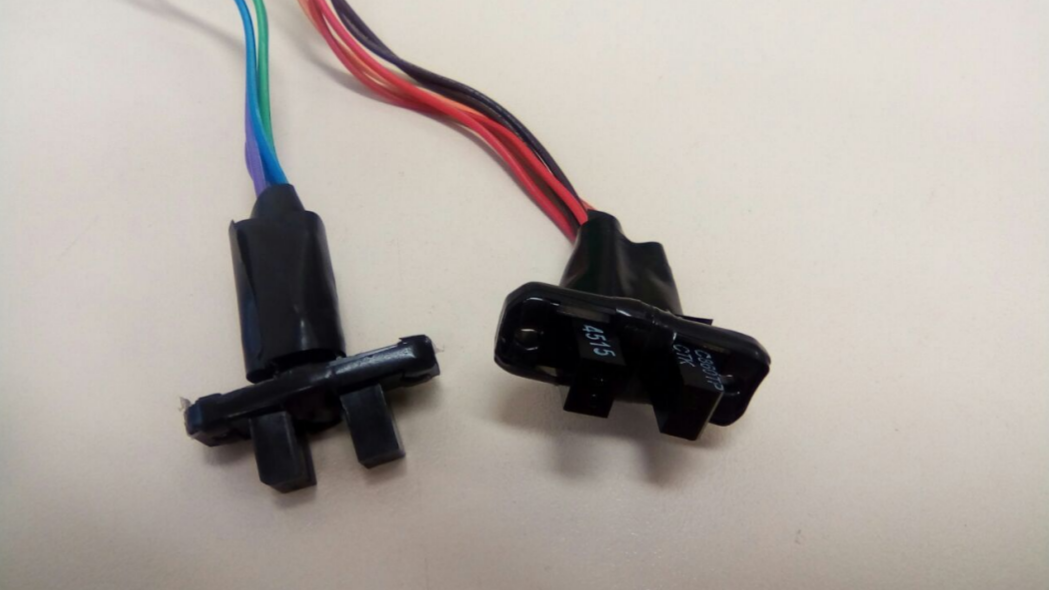
\includegraphics[width=9cm]{images/sensores1.png}
	\caption{Sensores Break Beam}
	\label{sensores1}
\end{figure}


\begin{figure}[!htb]
	\centering
	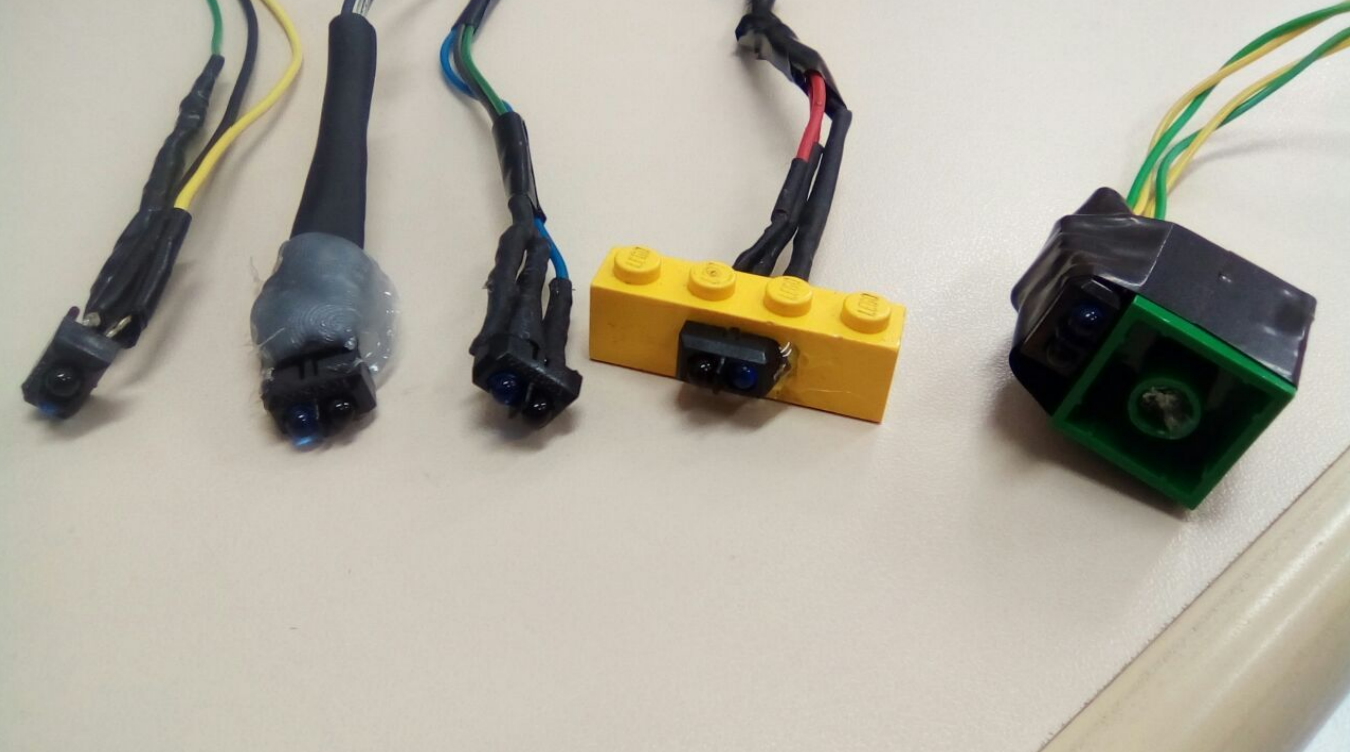
\includegraphics[width=9cm]{images/sensores2.png}
	\caption{Sensores Óptico Reflexivos}
	\label{sensores2}
\end{figure}

\begin{figure}[!htb]
	\centering
	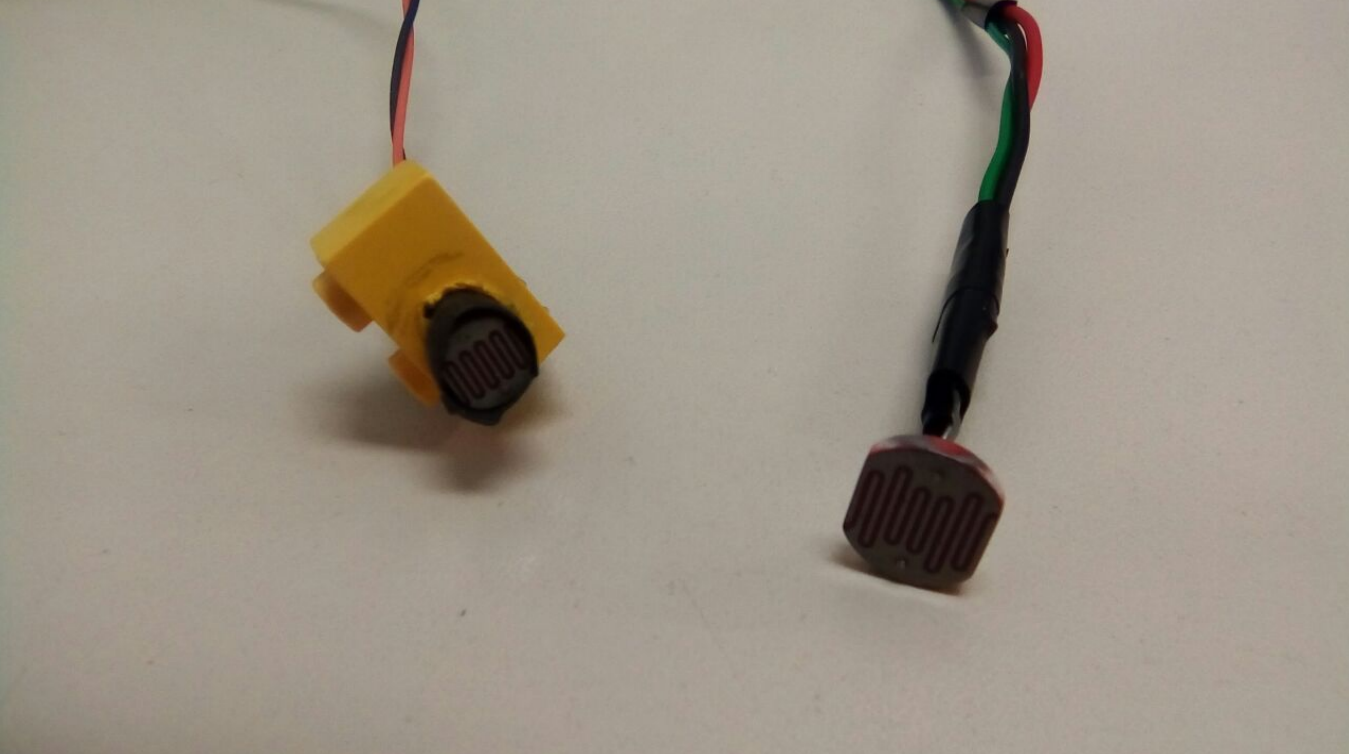
\includegraphics[width=9cm]{images/sensores3.png}
	\caption{Sensores LDR}
	\label{sensores3}
\end{figure}

\begin{figure}[!htb]
	\centering
	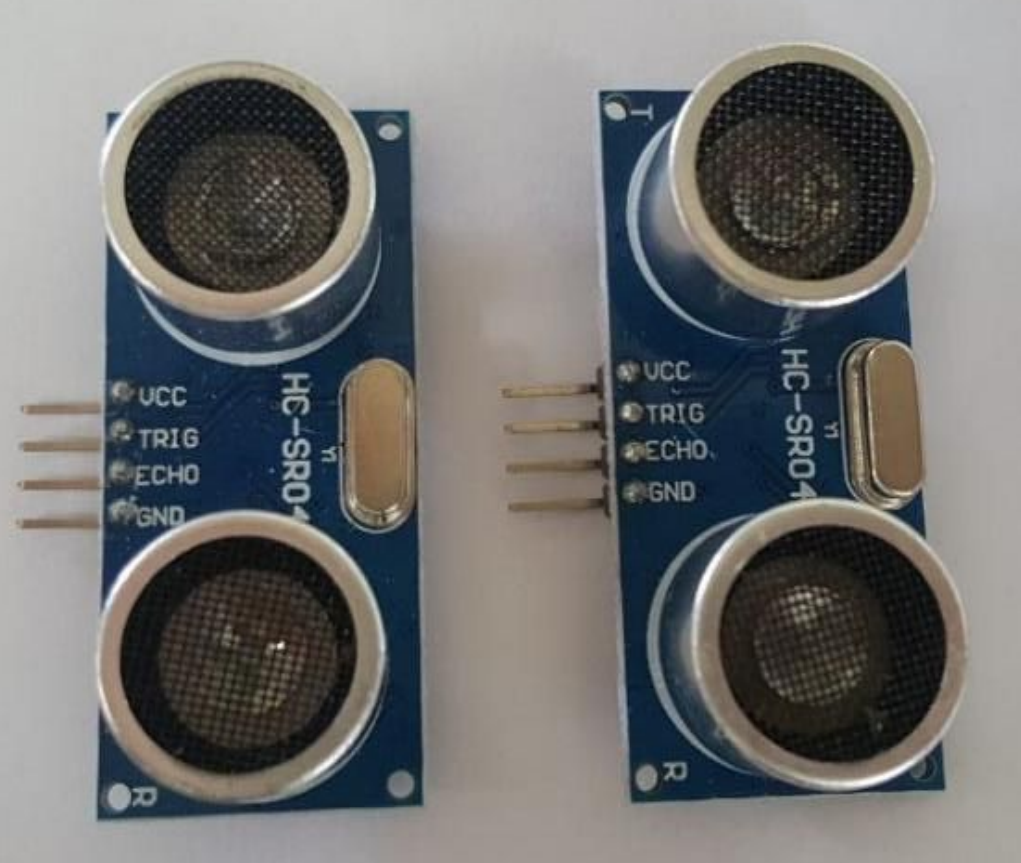
\includegraphics[width=7cm]{images/sensores4.png}
	\caption{Sensores Ultrassônicos}
	\label{sensores4}
\end{figure}

\begin{figure}[!htb]
	\centering
	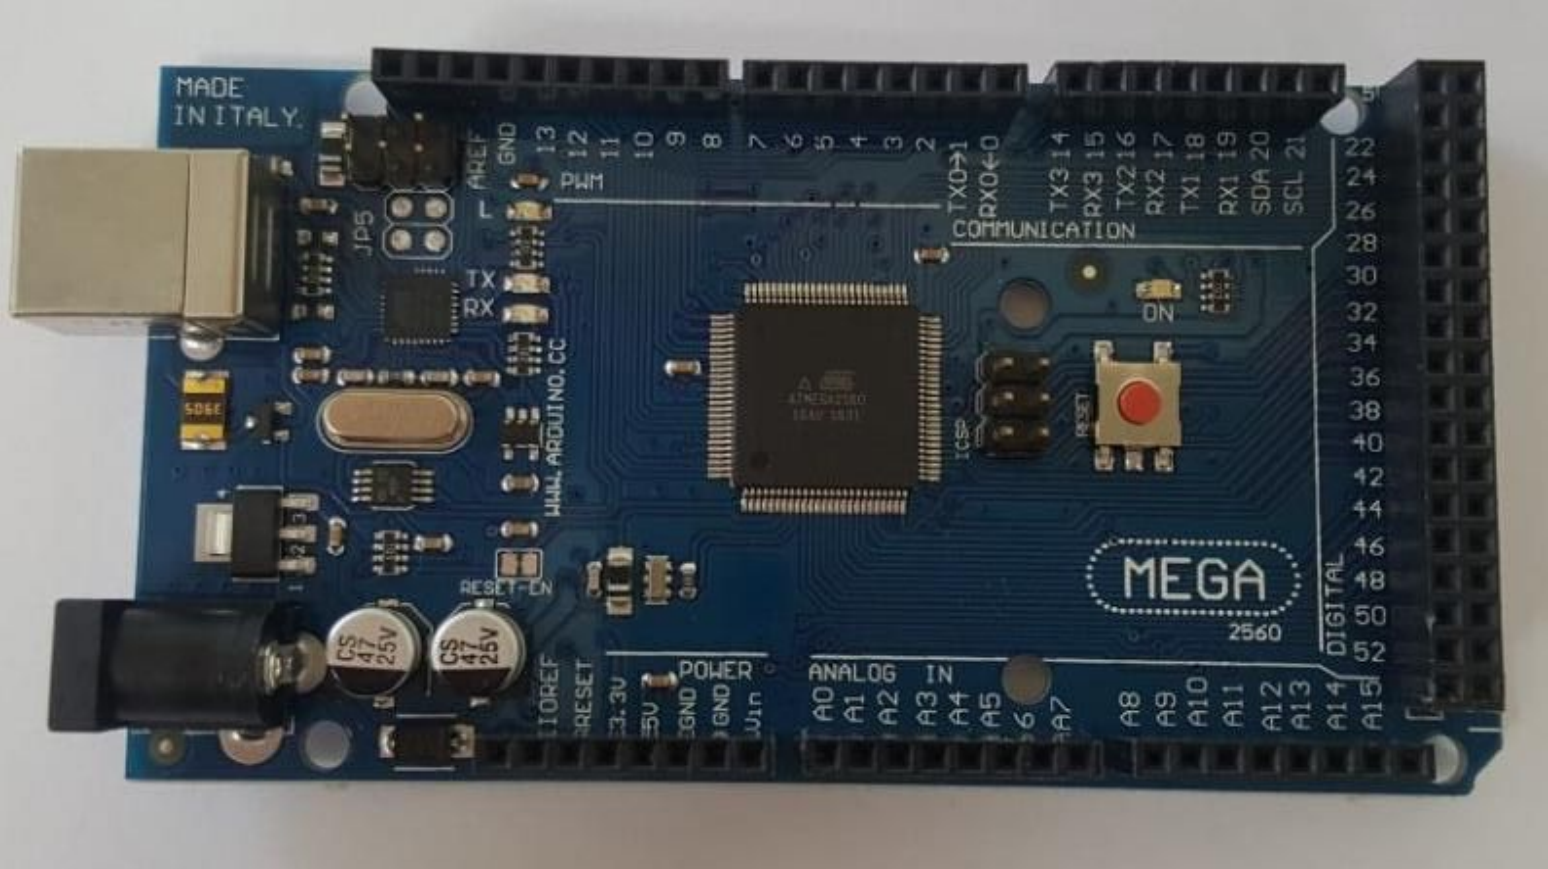
\includegraphics[width=8cm]{images/arduino.png}
	\caption{Plataforma Arduino}
	\label{arduino}
\end{figure}

\newpage

Para realizar o controle de motores com nossa placa Arduino, adquirimos um Motor Shield - Driver Ponte H (Figura \ref{shield}).

\begin{figure}[!htb]
	\centering
	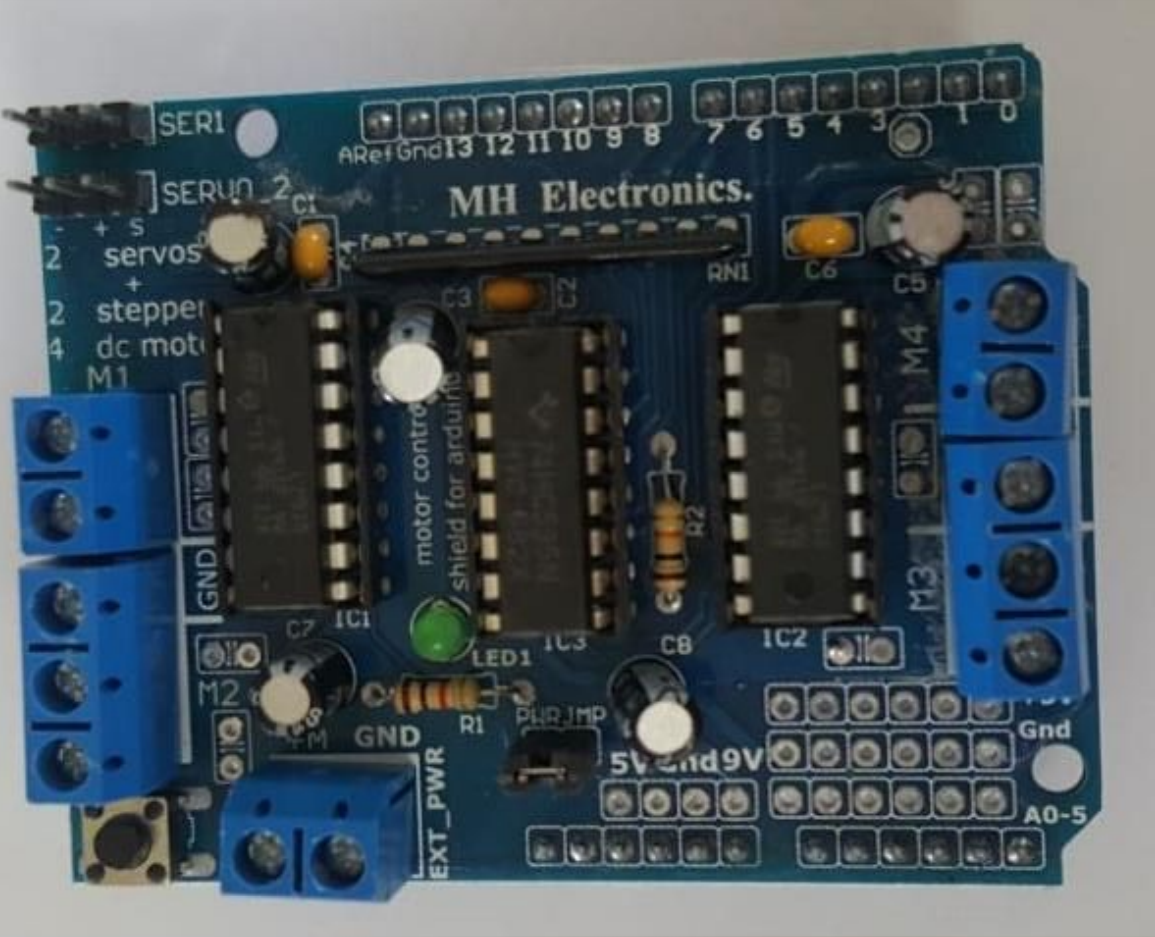
\includegraphics[width=8cm]{images/shield.png}
	\caption{Motor Shield - Driver Ponte H}
	\label{shield}
\end{figure}

\newpage

Após a montagem da estrutura e alocação dos sensores o robô ficou como mostrado na Figura \ref{robo}. 

\begin{figure}[!htb]
	\centering
	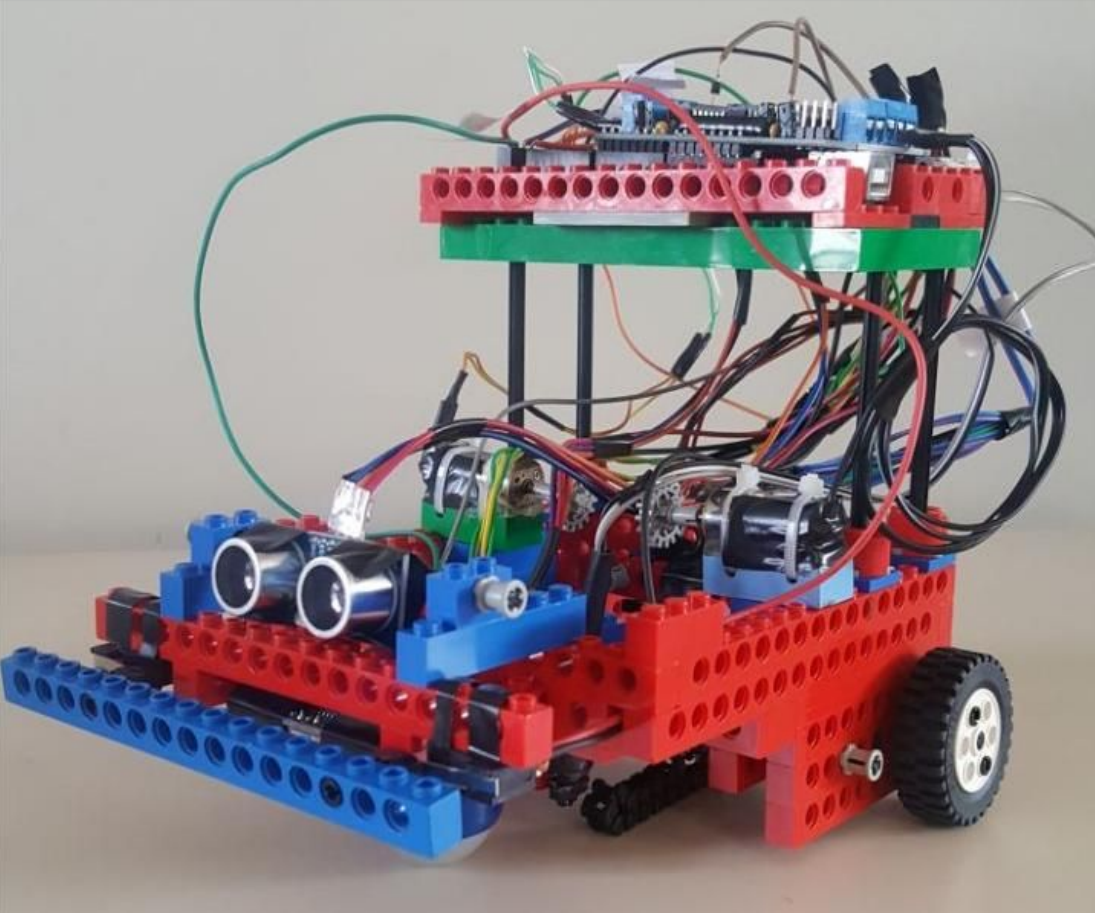
\includegraphics[width=10cm]{images/robo.png}
	\caption{Robô com estrutura finalizada.}
	\label{robo}
\end{figure}


\subsection{Métodos}

Para a montagem da estrutura do robô utilizamos o kit de Legos de forma a deixar o Arduíno, o Motor Shield e os sensores bem adaptados. Para a montagem e soldagem dos sensores nós utilizamos tutoriais ilustrados que podem ser facilmente obtidos na internet. Todos os sensores foram testados e apresentaram boa performance.

// Melhorar.
    
    \section{Tarefas do Robô}
    \label{sec:workProp}
    Nas duas subseções seguintes nós detalhamos as tarefas que o robô executará e como elas foram implementadas.

\subsection{Tarefas e Periodicidade}

Uma tarefa de tempo real, além da correção lógica, deve satisfazer seus prazos e restrições temporais. As restrições temporais, as relações de precedência e de exclusão usualmente impostas sobre tarefas são determinantes na definição de um modelo de tarefas que é parte integrante de um problema de escalonamento. 

Para que se tenha um comportamento temporal adequado, todas as tarefas de tempo real tipicamente estão sujeitas a prazos (deadlines). A princípio, uma tarefa deve ser concluída antes do seu deadline. As consequências de uma tarefa ser concluída após o seu deadline define dois tipos de tarefas de tempo real:

\begin{itemize}
	
	\item  \textbf{Tarefa Crítica}, quando ao ser completada depois de seu deadline pode causar falhas catastróficas no sistema de tempo real e em seu ambiente.
	
	\item \textbf{Tarefa Não-crítica}, quando ao ser completada depois de seu deadline no máximo implica numa diminuição de desempenho do sistema. 
	
\end{itemize}

Outra característica temporal de tarefas em sistemas de tempo real está baseada na periodicidade de suas atividades. Os modelos comportam dois tipos de tarefas neste aspecto, são eles:

\begin{itemize}
	
	\item \textbf{Tarefa Periódica}:  Tarefa que possui periodicidade de ativação (e não de execução) constante;
	
	\item \textbf{Tarefa Aperiódica}: Tarefa cujo intervalo de tempo entre ativações conse- cutivas não tem nenhum mínimo definido. Para poder ser considerada a utilização de tarefas aperiódicas em sistemas de tempo real, torna-se necessário impor um limite superior à sua utilização de recursos computacionais.
	
\end{itemize}

Na Tabela \ref{tabela} apresentamos as tarefas a serem implementadas juntamente com seus requisitos temporais.

\begin{table}[]
	\centering
	\caption{Tarefas e seus requisitos temporais}
	\label{tabela}
	\begin{tabular}{|c|l|c|c|c|}
		\hline
		\textbf{N°} & \multicolumn{1}{c|}{\textbf{Tarefa}}                                                            & \textbf{Modelo}                                                 & \textbf{\begin{tabular}[c]{@{}c@{}}Tempo de \\ Execução\\ (segundos)\end{tabular}} & \textbf{Prioridade} \\ \hline
		1           & Andar                                                                                           & \begin{tabular}[c]{@{}c@{}}Não crítica\\ Periódica\end{tabular} &                                                                                    &                     \\ \hline
		2           & Detectar e seguir uma linha                                                                     & \begin{tabular}[c]{@{}c@{}}Não crítica\\ Periódica\end{tabular} &                                                                                    &                     \\ \hline
		3           & Verificar obstáculo                                                                             & \begin{tabular}[c]{@{}c@{}}Não crítica\\ Periódica\end{tabular} &                                                                                    &                     \\ \hline
		4           & \begin{tabular}[c]{@{}l@{}}Manutenção da velocidade \\ utilizando um controle PID\end{tabular} & \begin{tabular}[c]{@{}c@{}}Não crítica\\ Periódica\end{tabular} &                                                                                    &                     \\ \hline
		5           & Verificar superície                                                                             & \begin{tabular}[c]{@{}c@{}}Não Crítica\\ Periódica\end{tabular} &                                                                                    &                     \\ \hline
		6           & \begin{tabular}[c]{@{}l@{}}Detectar contato com \\ objetos\end{tabular}                         & \begin{tabular}[c]{@{}c@{}}Não crítica\\ Periódica\end{tabular} &                                                                                    &                     \\ \hline
		7           & Desviar de obstáculos                                                                            & \begin{tabular}[c]{@{}c@{}}Crítica\\ Aperiódica\end{tabular}    &                                                                                    &                     \\ \hline
		8           & Evitar queda de superfícies                                                                     & \begin{tabular}[c]{@{}c@{}}Crítica\\ Aperiódica\end{tabular}    &                                                                                    &                     \\ \hline
		9           & \begin{tabular}[c]{@{}l@{}}Em caso de contato com \\ objeto, afastar do mesmo\end{tabular}     & \begin{tabular}[c]{@{}c@{}}Crítica\\ Aperiódica\end{tabular}    &                                                                                    &                     \\ \hline
	\end{tabular}
\end{table}

\newpage

\subsection{Implementação e Escalonamento das Tarefas}

Nesta seção mostraremos como as tarefas apresentadas na seção 3.1 foram implementadas. A primeira etapa foi verificar se existia algum algoritmo de escalonamento presente na literatura que se adaptasse ao nosso projeto. O algoritmo \textit{Rate Monotonic}, bastante conhecido, é um algoritmo que possui características que se adequam ao nosso projeto, portanto, usamos este algoritmo como base para implementação do nosso código.

As principais características do algoritmo \textit{Rate Monotonic} são:

\begin{itemize}
	
	\item As tarefas são periódicas e independentes;
	
	\item O deadline de cada tarefa coincide com o seu período;
	
	\item O tempo de computação de cada tarefa é conhecido e constante (\textit{Worst Case Computation Time});
	
	\item O tempo de chaveamento entre tarefas é assumido nulo;
	
	\item Dá maior prioridade às tarefas de menor período.
	
\end{itemize}

Nossas tarefas são em sua maioria periódicas, porém, três destas tarefas são aperiódicas. Para contornar esta situação e poder fazer uso do algoritmo \textit{Rate Monotonic} nós criamos um servidor de tarefas aperiódicas. Este servidor, é tratado como uma tarefa periódica. 

O algoritmo funciona da seguinte maneira: Todas as tarefas periódicas são executadas por tempo pré-definido, inclusive a tarefa referente ao servidor de aperiódicas. Para controle de execução das tarefa aperiódicas têm-se uma variável booleana global que auxilia para execução ou não de uma tarefa aperiódica. Este controle funciona da seguinte forma: Quando as tarefas \textbf{Verificar obstáculo}, \textbf{Detectar contato} e \textbf{Verificar superfície} são executadas elas retornam um valor. De acordo com o valor retornado, a variável booleana global  recebe o valor \textit{True} (por exemplo,  a variável booleana está setada como \textit{False}, se ao executar a tarefa de \textbf{Verificar obstáculo} o sensor apresentar um valor que é um valor de risco, esta variável recebe o valor \textit{True}), se ao ser executada a tarefa referente ao servidor de aperiódicos, a variável booleana estiver com valor \textit{True}, a tarefa aperiódica \textbf{Desviar de obstáculos} é executada. Ao final da execução da tarefa aperiódica, a variável booleana recebe o valor \textit{False} novamente.

//Melhorar
//Colocar pseudo-algoritmo



\section{Resultados}
	\label{sec:objetivos}
	Após o desenvolvimento do robô foram necessários vários testes para refinamento das tarefas, nós criamos uma pista para treino utilizando cartolinas e fita isolante. Isso possibilitou que as linhas pudessem ser trocadas com facilidade, o que nos permitiu ver o desempenho do robô em vários cenários.  Uma das pistas que montamos pode ser vista na Figura \ref{pista}, esta pista possui 94 cm de largura e 195 cm de altura.


//  Melhorar.

\begin{figure}[!htb]
	\centering
	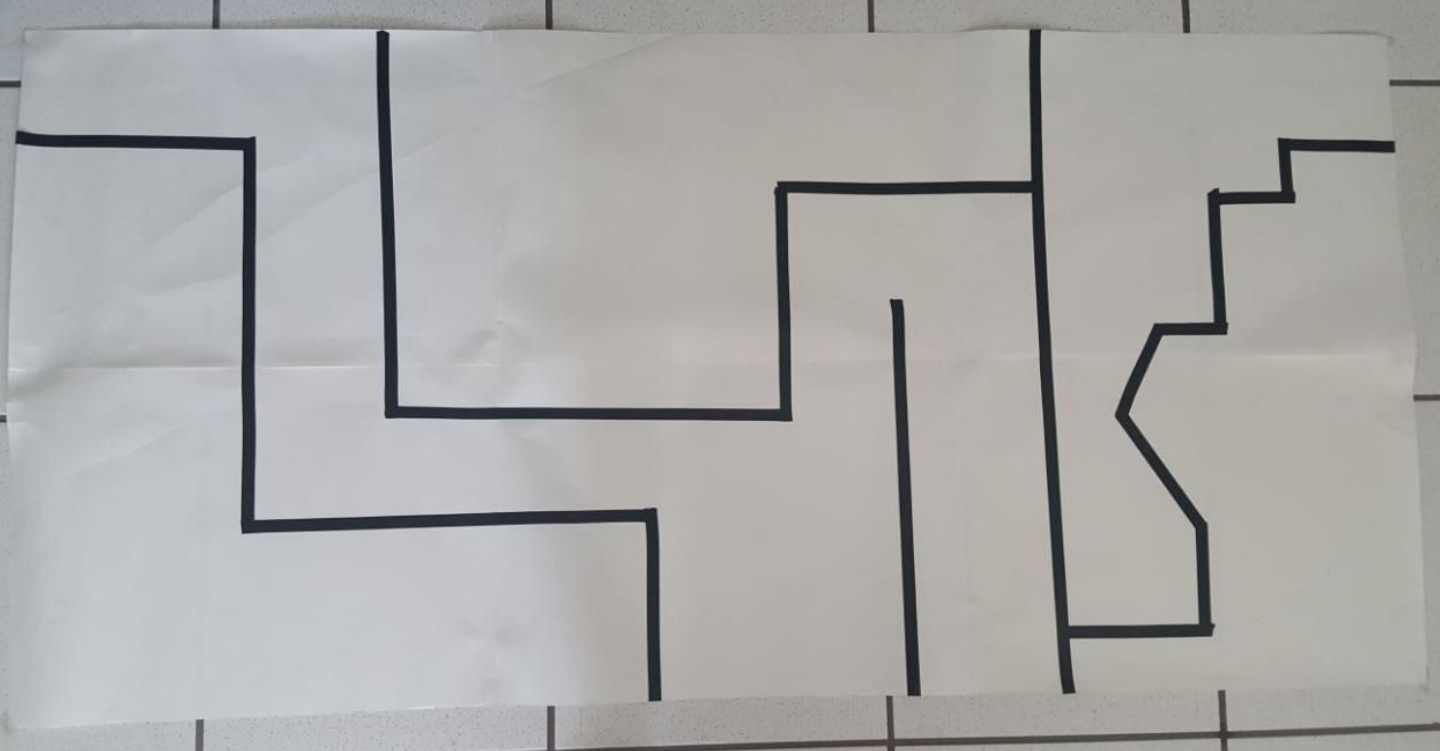
\includegraphics[width=10cm]{images/pista.png}
	\caption{Pista para testes.}
	\label{pista}
\end{figure}

\newpage

\section{Conclusão}
	\label{sec:materiais}
	Com este trabalho conseguimos aplicar nossos conhecimentos adquiridos durante o semestre e pudemos adquirir conhecimentos adicionais com os materiais e métodos utilizados para o desenvolvimento do projeto.  Sistemas de Tempo real geralmente são complexos devido às suas características de restrição temporal e sensibilidade à falhas, porém, devido ao grande planejamento que fizemos referente a implementação das tarefas e escalonamento, conseguimos desenvolver o robô de forma fluente, sem muitos contratempos. O robô apresentou resultado satisfatório apresentando bom desempenho na execução das tarefas propostas.

// Melhorar.
    

\newpage
\begin{thebibliography}{99}

\bibitem{farines}
    Farines, Jean-Marie, Joni da Silva Fraga, and RS de Oliveira. "Sistemas de tempo real." Escola de Computação 2000 (2000): 201.
    
\bibitem{PID}
Controle PID em sistemas embarcados. Carlos Márcio Freitas. Disponível em: www.embarcados.com.br/controle-pid-em-sistemas-embarcados. Acesso em: 23 ago. 2017.

    

\end{thebibliography}

\end{document}

